%% START FAVITES SUPPLEMENT
\chapter{Supplemental Material for Chapter~\ref{chap:favites}}
\label{chap:favites-sup}
\clearpage

%% Tables
\begin{table}[!ht] % TABLE S1 IN ORIGINAL PAPER
\caption[Comparison with Existing Simulation Tools]{Comparison with Existing Simulation Tools}
\vspace{-0.25in}
\begin{center}
\begin{tabular}{|P{0.8in}|P{0.5in}|P{0.8in}|P{0.8in}|P{0.6in}|P{0.8in}|P{0.8in}|}
\hline
 & \textbf{epinet} & \textbf{TreeSim} & \textbf{outbreaker} & \textbf{seedy} & \textbf{PANGEA} & \textbf{FAVITES} \\
\hline
\textbf{Contact Network} & Fixed & Complete & Complete & Complete & Fixed & Any \\
\hline
\textbf{Trans. Network} & Fixed & Fixed & Fixed & Fixed & Fixed & Any\\
\hline
\textbf{Sampling} & N/A & Fixed or \newline Sequential & Fixed & Uniform & Fixed & Any \\
\hline
\textbf{Phylogeny} & None & Fixed & Fixed & Fixed & Coalescent & Any \\
\hline
\textbf{Mutation Rate} & N/A & N/A & Constant & Constant & Fixed & Any \\
\hline
\textbf{Sequences} & None & None & Fixed & Fixed & Fixed & Any \\
\hline
\textbf{Sequencing} & N/A & N/A & No & No & No & Any \\
\hline
\end{tabular}
\end{center}
\label{tab:favites-comparison}
\end{table}

\begin{table}[!ht] % TABLE S2 IN ORIGINAL PAPER
\caption[Post-Validation Tools]{Post-Validation Tools}
\vspace{-0.25in}
\begin{center}
\begin{tabular}{|P{2.3in}|P{3.7in}|}
\hline
\textbf{Name} & \textbf{Description}  \\
\hline
compare\_contact\_networks.py & Compare the degree distributions of a given simulated contact network against a reference contact network \\
\hline
compare\_trees.py & Compare the distributions of all branch lengths, internal branch lengths, terminal branch lengths, and root-to-tip distances between a given simulated tree against a given reference tree \\
\hline
distribution\_distance.py & Compute a distance between two distributions given samples from each \\
\hline
ltt.py & Create a \gls{LTT} plot from one or more Newick trees \\
\hline
sequence\_score\_profile\_HMM.py & Score a given sequence dataset against a given profile \gls{HMM} \\
\hline
\end{tabular}
\end{center}
\label{tab:favites-post-validation}
\end{table}

\begin{table}[!ht] % TABLE S3 IN ORIGINAL PAPER
\caption[Helper Scripts]{Helper Scripts}
\vspace{-0.25in}
\begin{center}
\begin{tabular}{|P{2.75in}|P{3.25in}|}
\hline
\textbf{Name} & \textbf{Description}  \\
\hline
clean\_labels.py & For each read of the given sequence file or each leaf of a given phylogenetic tree, remove everything from the label except for the contact network individual's name \\
\hline
cluster\_previous\_time.py & Given a clustering from the simulation end time, a FAVITES-format transmission network, and a time, remove individuals who were not infected at the given time and output the resulting clusters \\
\hline
cn\_adjacency\_matrix\_to\_favites.py & Convert a given contact network from a binary adjacency matrix to the FAVITES format \\
\hline
degree\_stats.py & Given a contact or transmission network, compute various statistics of the node degree distribution \\
\hline
FAVITES2GEXF.py & Convert a FAVITES contact network and transmission network to the GEXF format \\
\hline
PANGEA\_transmissions\_to\_FAVITES.py & Convert a PANGEA transmission network into the FAVITES edge-list format \\
\hline
patristic\_distances.py & Given a phylogenetic tree, compute the pairwise distances between leaves and output the resulting distance matrix as a CSV file \\
\hline
scale\_tree.py & Given a phylogenetic tree (in the Newick format), scale all branches \\
\hline
score\_clusters.py & Score a given query clustering against a given true reference clustering \\
\hline
tn93\_to\_clusters.py & Convert tn93 output to the Cluster Picker clustering format \\
\hline
\end{tabular}
\end{center}
\label{tab:favites-helper}
\end{table}

\begin{table}[!ht] % TABLE S4 IN ORIGINAL PAPER
\caption[Simulation Parameters: Epidemiological Model]{HIV Simulation Parameters (epidemiological model)}
\vspace{-0.25in}
\begin{center}
\begin{tabular}{|P{2in}|P{1.9in}|P{1.9in}|}
\hline
 & \textbf{San Diego} & \textbf{Uganda} \\
\hline
\textbf{CN Model} & \gls{BA} & \gls{BA} \\
\hline
\textbf{Expected Degree} & 4 & 4 \\
\hline
\textbf{Number of Seeds} & 1,500 & 15,000 \\
\hline
\textbf{$\lambda_{AU\rightarrow CU}$} (year$^{-1}$) & 8.667 & 8.667 \\
\hline
\textbf{$\lambda_{AT\rightarrow CT}$} (year$^{-1}$) & 4.333 & 4.333 \\
\hline
\textbf{$\lambda_{U\rightarrow T}$} (year$^{-1}$) & 1 & 1 \\
\hline
\textbf{$\lambda_{T\rightarrow U}$} (year$^{-1}$) & 1 & 0.48 \\
\hline
\textbf{$\lambda_{S,AU}$} (year$^{-1}$) & 0.1125 & 0.1125 \\
\hline
\textbf{$\lambda_{S,AC}$} (year$^{-1}$) & 0.0225 & 0.0225 \\
\hline
\textbf{$\lambda_{S,AT}$} (year$^{-1}$) & 0.005625 & 0.005625 \\
\hline
\textbf{$\lambda_{S,CT}$} (year$^{-1}$) & 0 & 0 \\
\hline
%\textbf{Rate from Acute Treated to Chronic Treated} & 
\end{tabular}
\end{center}
\label{tab:favites-params-epi}
\end{table}

\begin{table}[!ht] % TABLE S5 IN ORIGINAL PAPER
\caption[Simulation Parameters: Evolutionary Model]{HIV Simulation Parameters (evolutionary model)}
\vspace{-0.25in}
\begin{center}
\begin{tabular}{|P{2in}|P{1.9in}|P{1.9in}|}
\hline
 & \textbf{San Diego} & \textbf{Uganda} \\
\hline
\textbf{Seed Height} (years) & 25 & 25 \\
\hline
\textbf{Seed Rate} & $1 + e^{-t^2}$ & $1 + e^{-t^2}$ \\
\hline
\textbf{Population Growth} & 2.852 & 2.852 \\
\hline
\textbf{v.T50} & -2 & -2 \\
\hline
\textbf{Mutation Rate Location} & 0.0008 & 0.001 \\
\hline
\textbf{Mutation Rate Scale} & 0.0005 & 0.0005 \\
\hline
\textbf{\gls{GTR} $\pi_A$} & 0.392 & 0.377 \\
\hline
\textbf{\gls{GTR} $\pi_C$} & 0.164 & 0.172 \\
\hline
\textbf{\gls{GTR} $\pi_G$} & 0.212 & 0.210 \\
\hline
\textbf{\gls{GTR} $\pi_T$} & 0.232 & 0.241 \\
\hline
\textbf{\gls{GTR} $\pi_{AC}$} & 1.812 & 1.388 \\
\hline
\textbf{\gls{GTR} $\pi_{AG}$} & 9.934 & 7.017 \\
\hline
\textbf{\gls{GTR} $\pi_{AT}$} & 0.718 & 0.736 \\
\hline
\textbf{\gls{GTR} $\pi_{CG}$} & 0.971 & 0.594 \\
\hline
\textbf{\gls{GTR} $\pi_{CT}$} & 9.934 & 8.618 \\
\hline
\textbf{\gls{GTR} $\pi_{GT}$} & 1 & 1 \\
\hline
\textbf{$\alpha$} ($\Gamma$ shape) & 0.405 & 0.449 \\
\hline
\end{tabular}
\end{center}
\label{tab:favites-params-evo}
\end{table}

\begin{table}[!ht] % TABLE S6 IN ORIGINAL PAPER
\caption[Real vs. Simulated \gls{JSD}]{Real vs. Simulated \gls{JSD}. All columns except the last (UG; for Uganda) correspond to the San Diego simulations. \gls{JSD} is computed between two distributions, one based on real data and one based on simulated data (either using true trees or trees inferred using IQ-TREE from simulated data). Distributions correspond to pairwise leaf distances on the tree (patristic distance), branch lengths (BL), and pairwise sequence distances corrected using \gls{JC69}+$\Gamma$ correction (see Fig.~\ref{fig:favites-dist-kde}).}
\vspace{-0.25in}
\begin{center}
\begin{tabular}{|c|c|c|c|c|c|}
\hline
 & True Patristic & Inferred Patristic & True BL & Inferred BL & \gls{JC69}+$\Gamma$ \\
\hline
\EART$=8$ & 0.195 & 0.027 & 0.050 & 0.100 & 0.049 \\
\hline
\EART$=4$ & 0.189 & 0.025 & 0.052 & 0.111 & 0.045 \\
\hline
\EART$=2$ & 0.193 & 0.033 & 0.045 & 0.097 & 0.035 \\
\hline
\textbf{Base} & 0.202 & 0.023 & 0.044 & 0.102 & 0.024 \\
\hline
\EART$=\frac{1}{2}$ & 0.188 & 0.023 & 0.057 & 0.116 & 0.040 \\
\hline
\EART$=\frac{1}{4}$ & 0.202 & 0.018 & 0.047 & 0.110 & 0.027 \\
\hline
\EART$=\frac{1}{8}$ & 0.163 & 0.024 & 0.046 & 0.103 & 0.023 \\
\hline
\ED$=2$ & 0.183 & 0.024 & 0.108 & 0.043 & 0.042 \\
\hline
\ED$=8$ & 0.179 & 0.025 & 0.103 & 0.056 & 0.033 \\
\hline
\ED$=16$ & 0.196 & 0.035 & 0.108 & 0.053 & 0.034 \\
\hline
\textbf{UG} & 0.100 & 0.082 & 0.082 & 0.119 & 0.243 \\
\hline
\end{tabular}
\end{center}
\label{tab:favites-jsd}
\end{table}

\begin{table}[!ht] % TABLE S7 IN ORIGINAL PAPER
\caption[Summary of Simulation Results]{Simulation Result Summary. U:T denotes the ratio of untreated to treated individuals.}
\vspace{-0.25in}
\begin{center}
\begin{tabular}{|c|c|c|c|c|}
\hline
\textbf{Condition} & \textbf{U:T} & \textbf{Prop. Inf. Increase} & \textbf{\gls{RF} Distance} & \textbf{Prop. Short} \\
\hline
Base & $0.507 \pm 0.004$ & $1.449 \pm 0.005$ & $0.430 \pm 0.052$ & $0.203 \pm 0.015$ \\
\hline
\EART$=\frac{1}{8}$ & $0.061 \pm 0.001$ & $1.086 \pm 0.003$ & $0.452 \pm 0.032$ & $0.193 \pm 0.012$ \\
\hline
\EART$=\frac{1}{4}$ & $0.122 \pm 0.002$ & $1.150 \pm 0.004$ & $0.481 \pm 0.042$ & $0.199 \pm 0.012$ \\
\hline
\EART$=\frac{1}{2}$ & $0.248 \pm 0.004$ & $1.127 \pm 0.005$ & $0.465 \pm 0.040$ & $0.207 \pm 0.014$ \\
\hline
\EART$=2$ & $1.036 \pm 0.013$ & $1.677 \pm 0.019$ & $0.429 \pm 0.027$ & $0.210 \pm 0.009$ \\
\hline
\EART$=4$ & $2.122 \pm 0.019$ & $1.885 \pm 0.008$ & $0.437 \pm 0.034$ & $0.218 \pm 0.013$ \\
\hline
\EART$=8$ & $4.289 \pm 0.047$ & $2.034 \pm 0.012$ & $0.433 \pm 0.041$ & $0.220 \pm 0.013$ \\
\hline
\ED$=2$ & $0.499 \pm 0.007$ & $1.196 \pm 0.006$ & $0.516 \pm 0.038$ & $0.199 \pm 0.010$ \\
\hline
\ED$=8$ & $0.531 \pm 0.009$ & $2.103 \pm 0.013$ & $0.434 \pm 0.031$ & $0.234 \pm 0.010$ \\
\hline
\ED$=16$ & $0.537 \pm 0.005$ & $3.586 \pm 0.017$ & $0.487 \pm 0.019$ & $0.283 \pm 0.005$ \\
\hline
\gls{ER} & $0.503 \pm 0.006$ & $1.359 \pm 0.007$ & $0.384 \pm 0.039$ & $0.186 \pm 0.015$ \\
\hline
\gls{WS} & $0.504 \pm 0.007$ & $1.337 \pm 0.005$ & $0.370 \pm 0.047$ & $0.180 \pm 0.011$ \\
\hline
Edge-Weighted & $0.511 \pm 0.005$ & $1.571 \pm 0.007$ & $0.409 \pm 0.025$ & $0.209 \pm 0.009$ \\
\hline
Uganda & $1.041 \pm 0.046$ & $1.639 \pm 0.027$ & $0.297 \pm 0.042$ & $0.185 \pm 0.021$ \\
\hline
\end{tabular}
\end{center}
\label{tab:favites-sim-results}
\end{table}

%% Figures
\begin{figure} % FIGURE S1 IN ORIGINAL PAPER
\centering
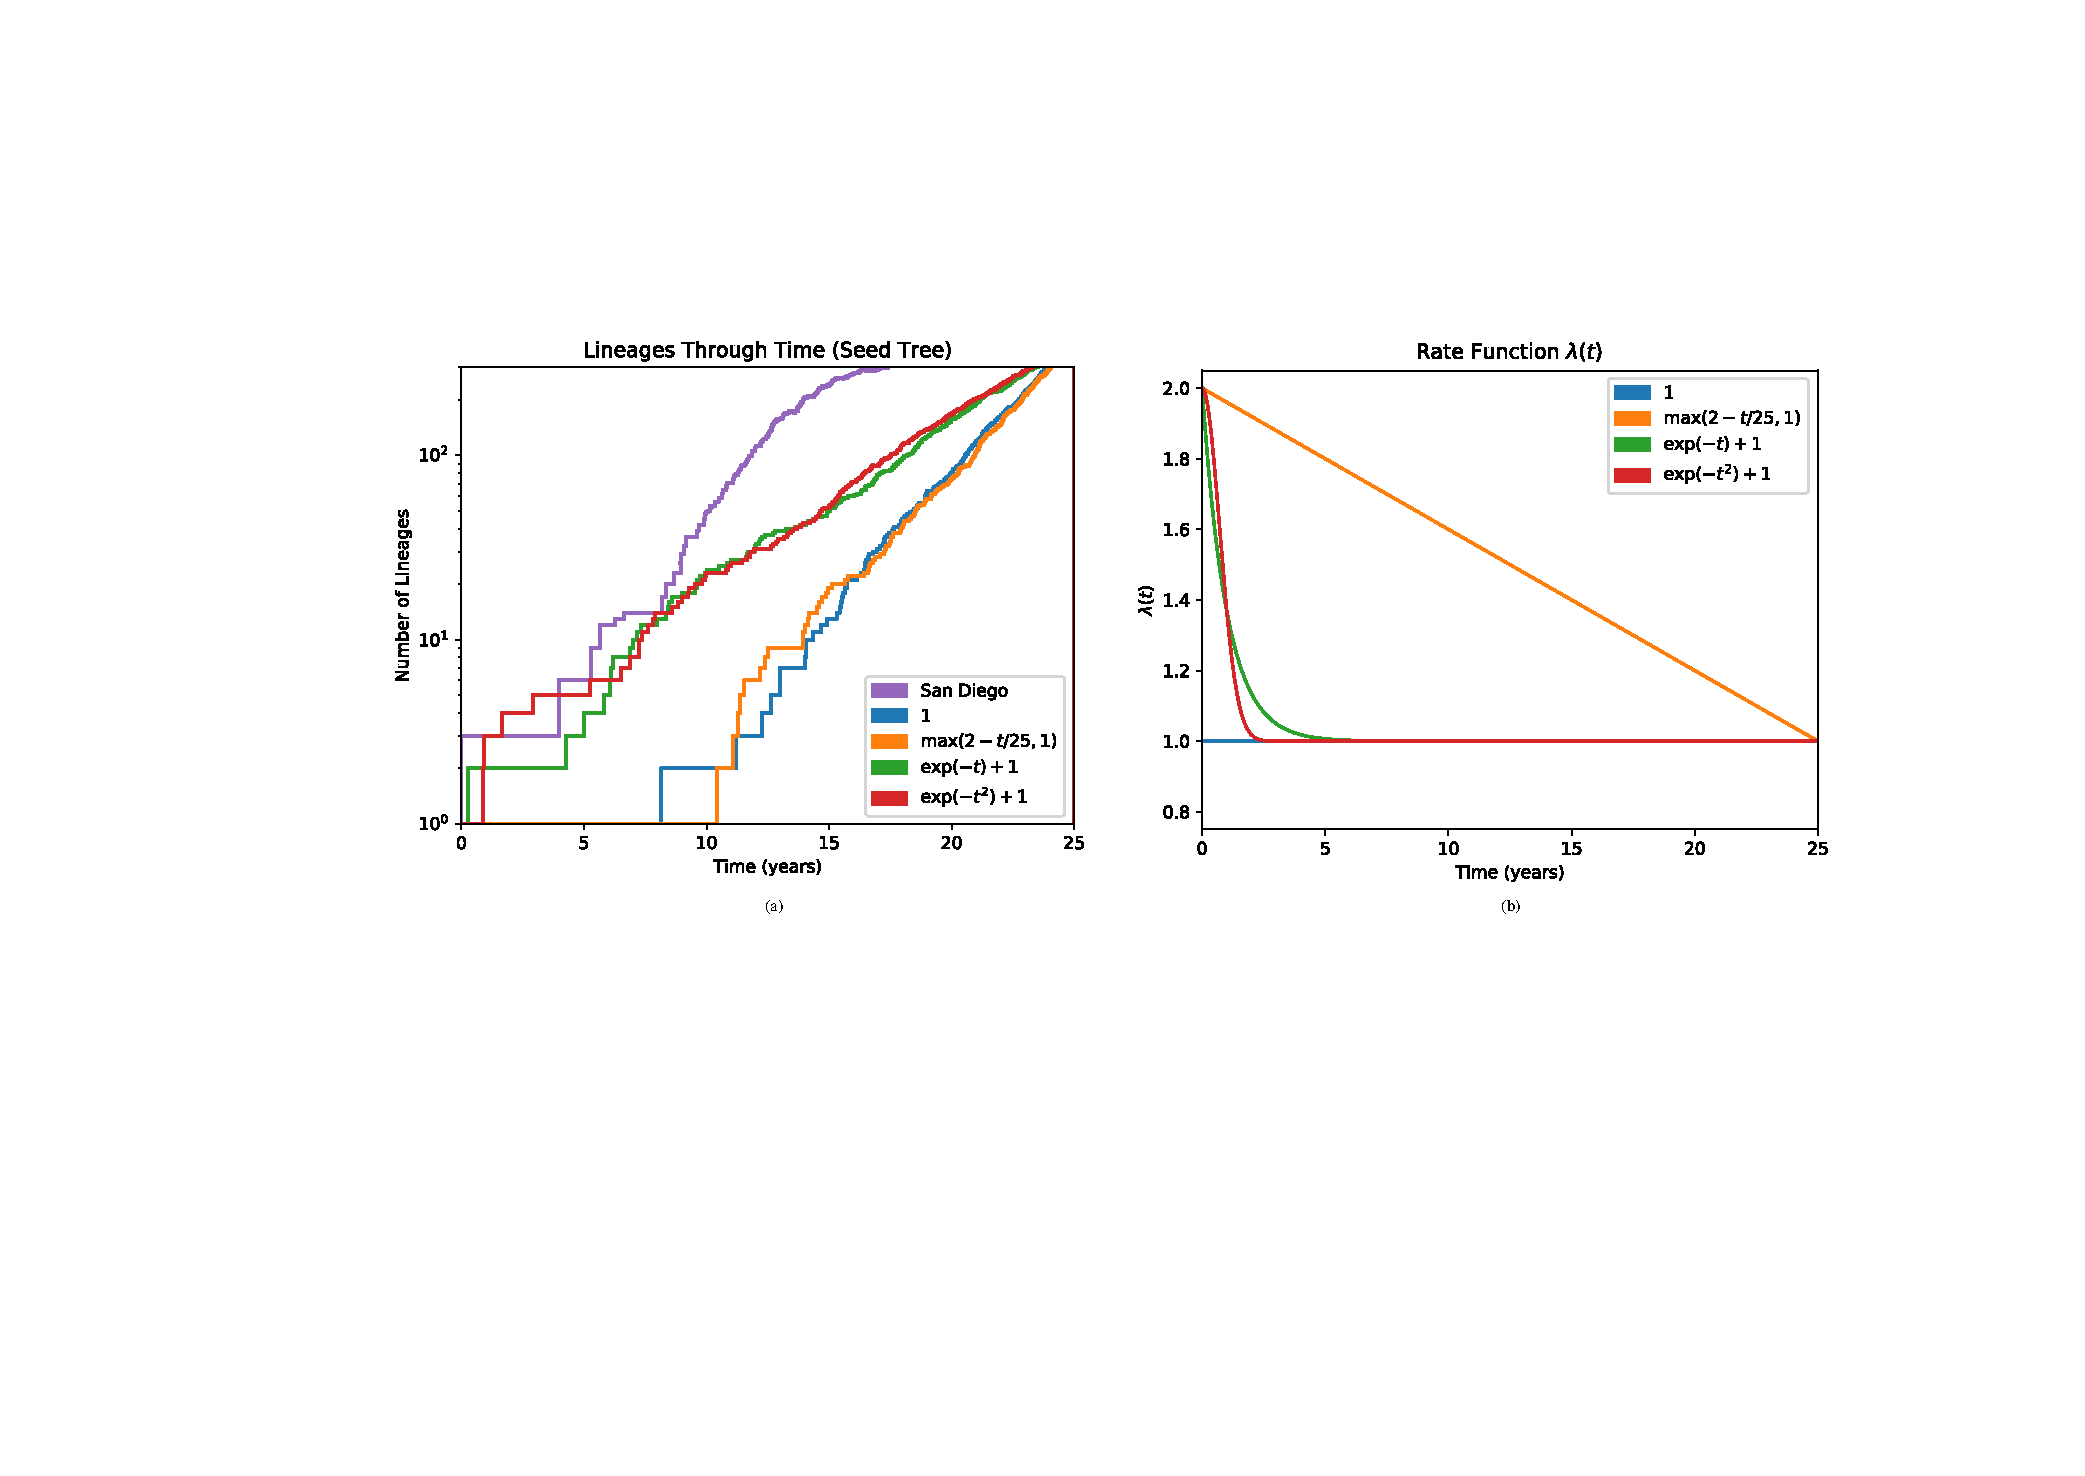
\includegraphics[width=\textwidth]{figs/favites-seed-tree}
\caption[Seed Tree]
{(a) \gls{LTT} plot of the first 25 years of the dated San Diego tree along with multiple potential rate functions for the non-homogeneous Yule model~\cite{LeGat2016}, and (b) plots of the rate functions. Because HIV trees have more short branches than normal Yule models (i.e., rate 1), we looked for functions that lead to increased numbers of lineages close to the root. This can be done by increasing the rate close to the root and then gradually decreasing the rate. As can be seen, $\lambda(t)=1$ and $\lambda(t)=\max(2-t/25,1)$ are far lower than the real San Diego curve. $\lambda(t)=\exp(-t)+1$ is much closer to the real curve, and $\lambda(t)=\exp(-t^2)+1$ is marginally closer than it. We chose to use $\lambda(t)=\exp(-t^2)+1$ as a result.}
\label{fig:favites-seed-tree}
\end{figure}

\begin{figure} % FIGURE S3 IN ORIGINAL PAPER
\centering
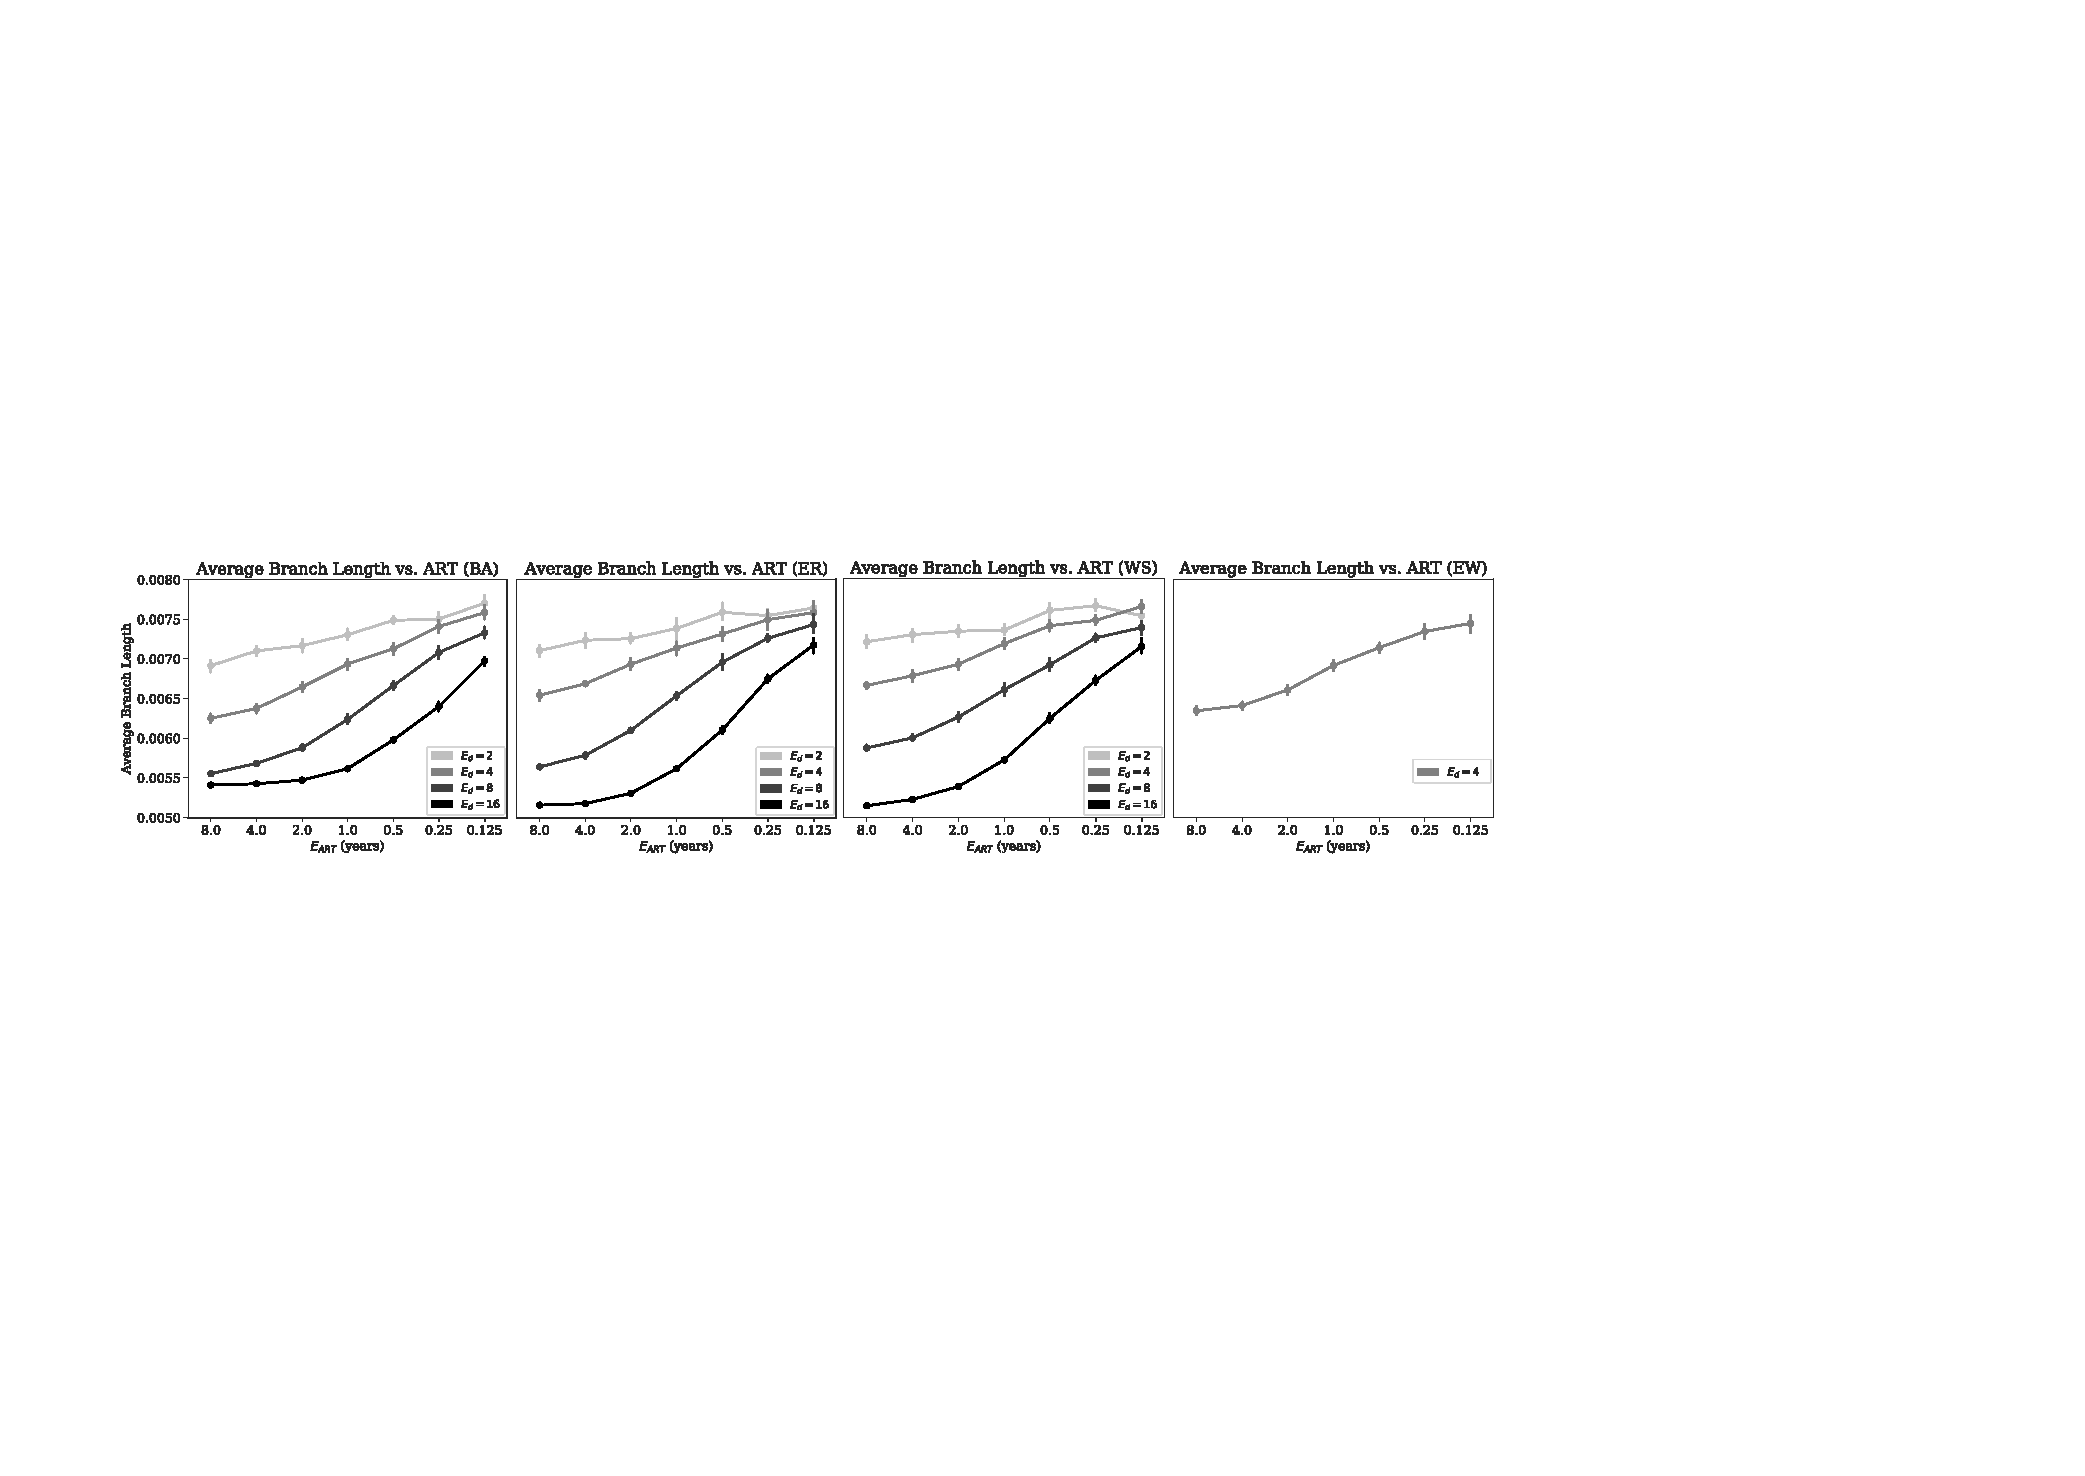
\includegraphics[width=\textwidth]{figs/favites-avg-bl-vs-art}
\caption[Average Branch Length vs. Expected Treatment Initiation Time]
{Average true branch length vs. \EART for the \gls{BA}, \gls{ER}, and \gls{WS} models with random seed selection as well as for the \gls{BA} model with edge-weighted seed selection with various expected degrees. The base parameters were chosen for all other parameters.}
\label{fig:favites-avg-bl-vs-art}
\end{figure}

\begin{figure} % FIGURE S4 IN ORIGINAL PAPER
\centering
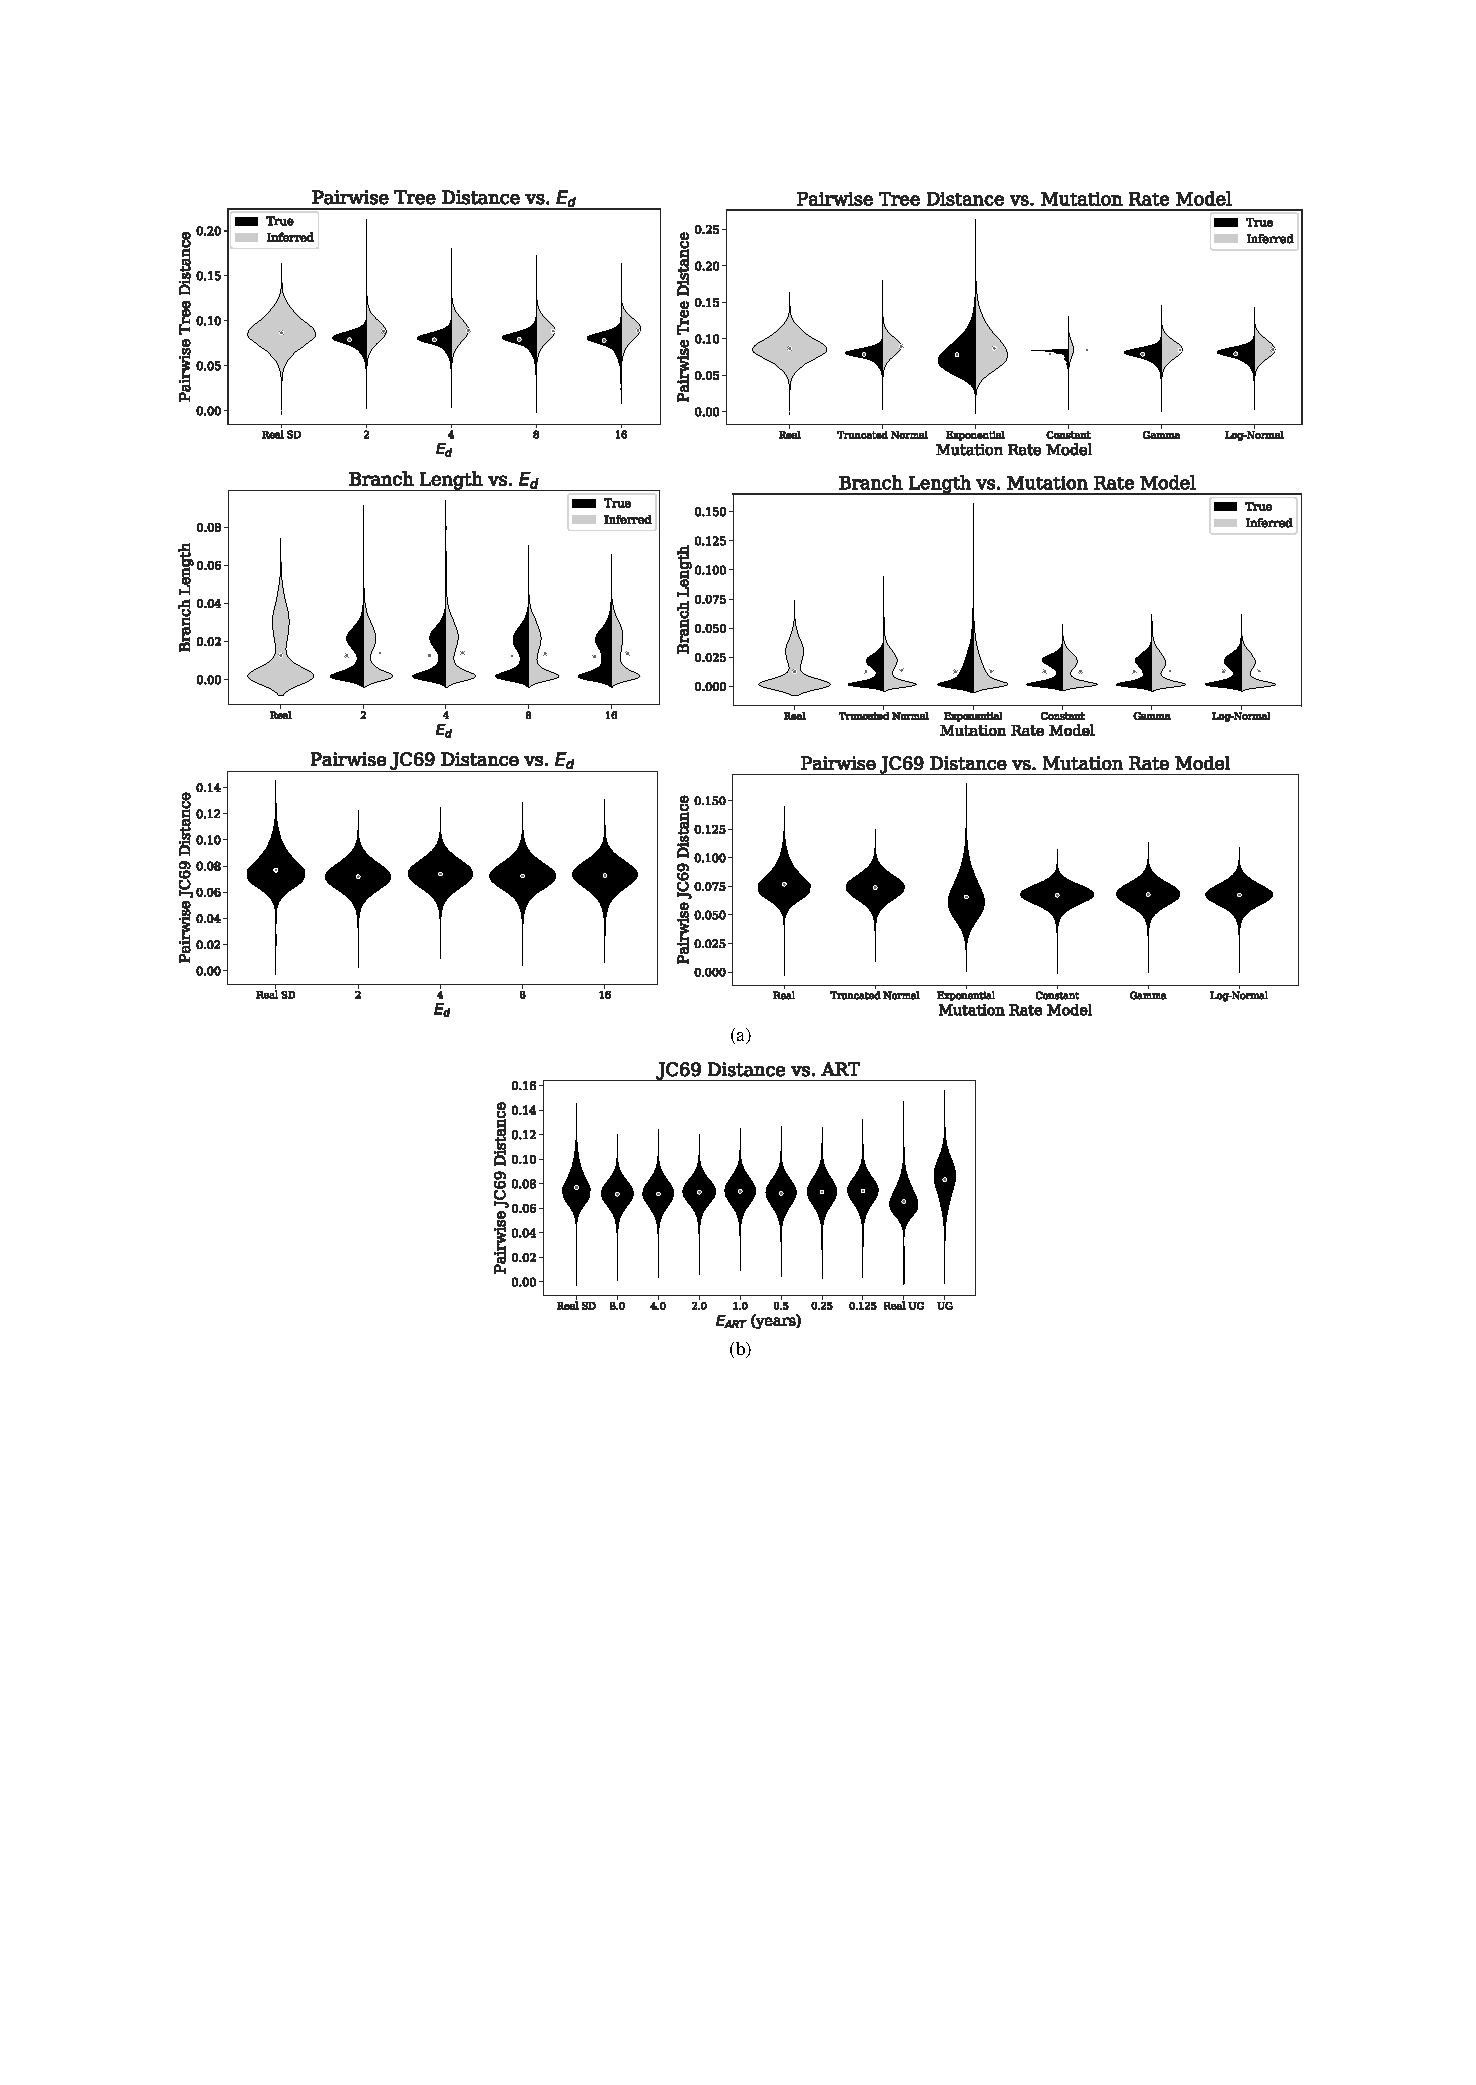
\includegraphics[width=0.8\textwidth]{figs/favites-dist-kde}
\caption[Branch Length and Pairwise Distance Distributions]
{(a) Kernel density estimates of the distributions of (Top) pairwise tree distances, (Middle) branch lengths, and (Bottom) pairwise \gls{JC69}+$\Gamma$ distances of real and simulated datasets for San Diego and Uganda using the default value of \EART$=1$ year for (Left) various values of \ED and (Right) various mutation rate models. For a pair of sequences with Hamming distance $d$, the phylogenetic distance corrected under the \gls{JC69}+$Gamma$ model is $t=\frac{3\alpha}{4}\left(\left(1-\frac{4d}{3}\right)^{-\frac{1}{\alpha}}-1\right)$, where $\alpha$ is the shape parameter of the Gamma distribution and is estimated using IQ-TREE~\cite{Chernomor2016} in \gls{JC69}+$\Gamma$ mode. The \gls{JSD} between the distributions of each model and the real dataset distributions are as follows: for inferred pairwise distances, Truncated Normal = 0.023, Exponential = 0.055, Constant = 0.059, Gamma = 0.031, and Log-Normal = 0.024; for inferred branch length, Truncated Normal = 0.044, Exponential = 0.031, Constant = 0.072, Gamma = 0.054, and Log-Normal = 0.059. Overall, truncated normal and log-normal distributions have the best match. The \gls{JSD} values for the distributions in which \ED is varied can be found in Table~\ref{tab:favites-jsd}. (b) Kernel density estimates of distributions of pairwise \gls{JC69}+$\Gamma$ distances on San Diego simulations with various \EART values and for Uganda.}
\label{fig:favites-dist-kde}
\end{figure}

\begin{figure} % FIGURE S2 IN ORIGINAL PAPER
\centering
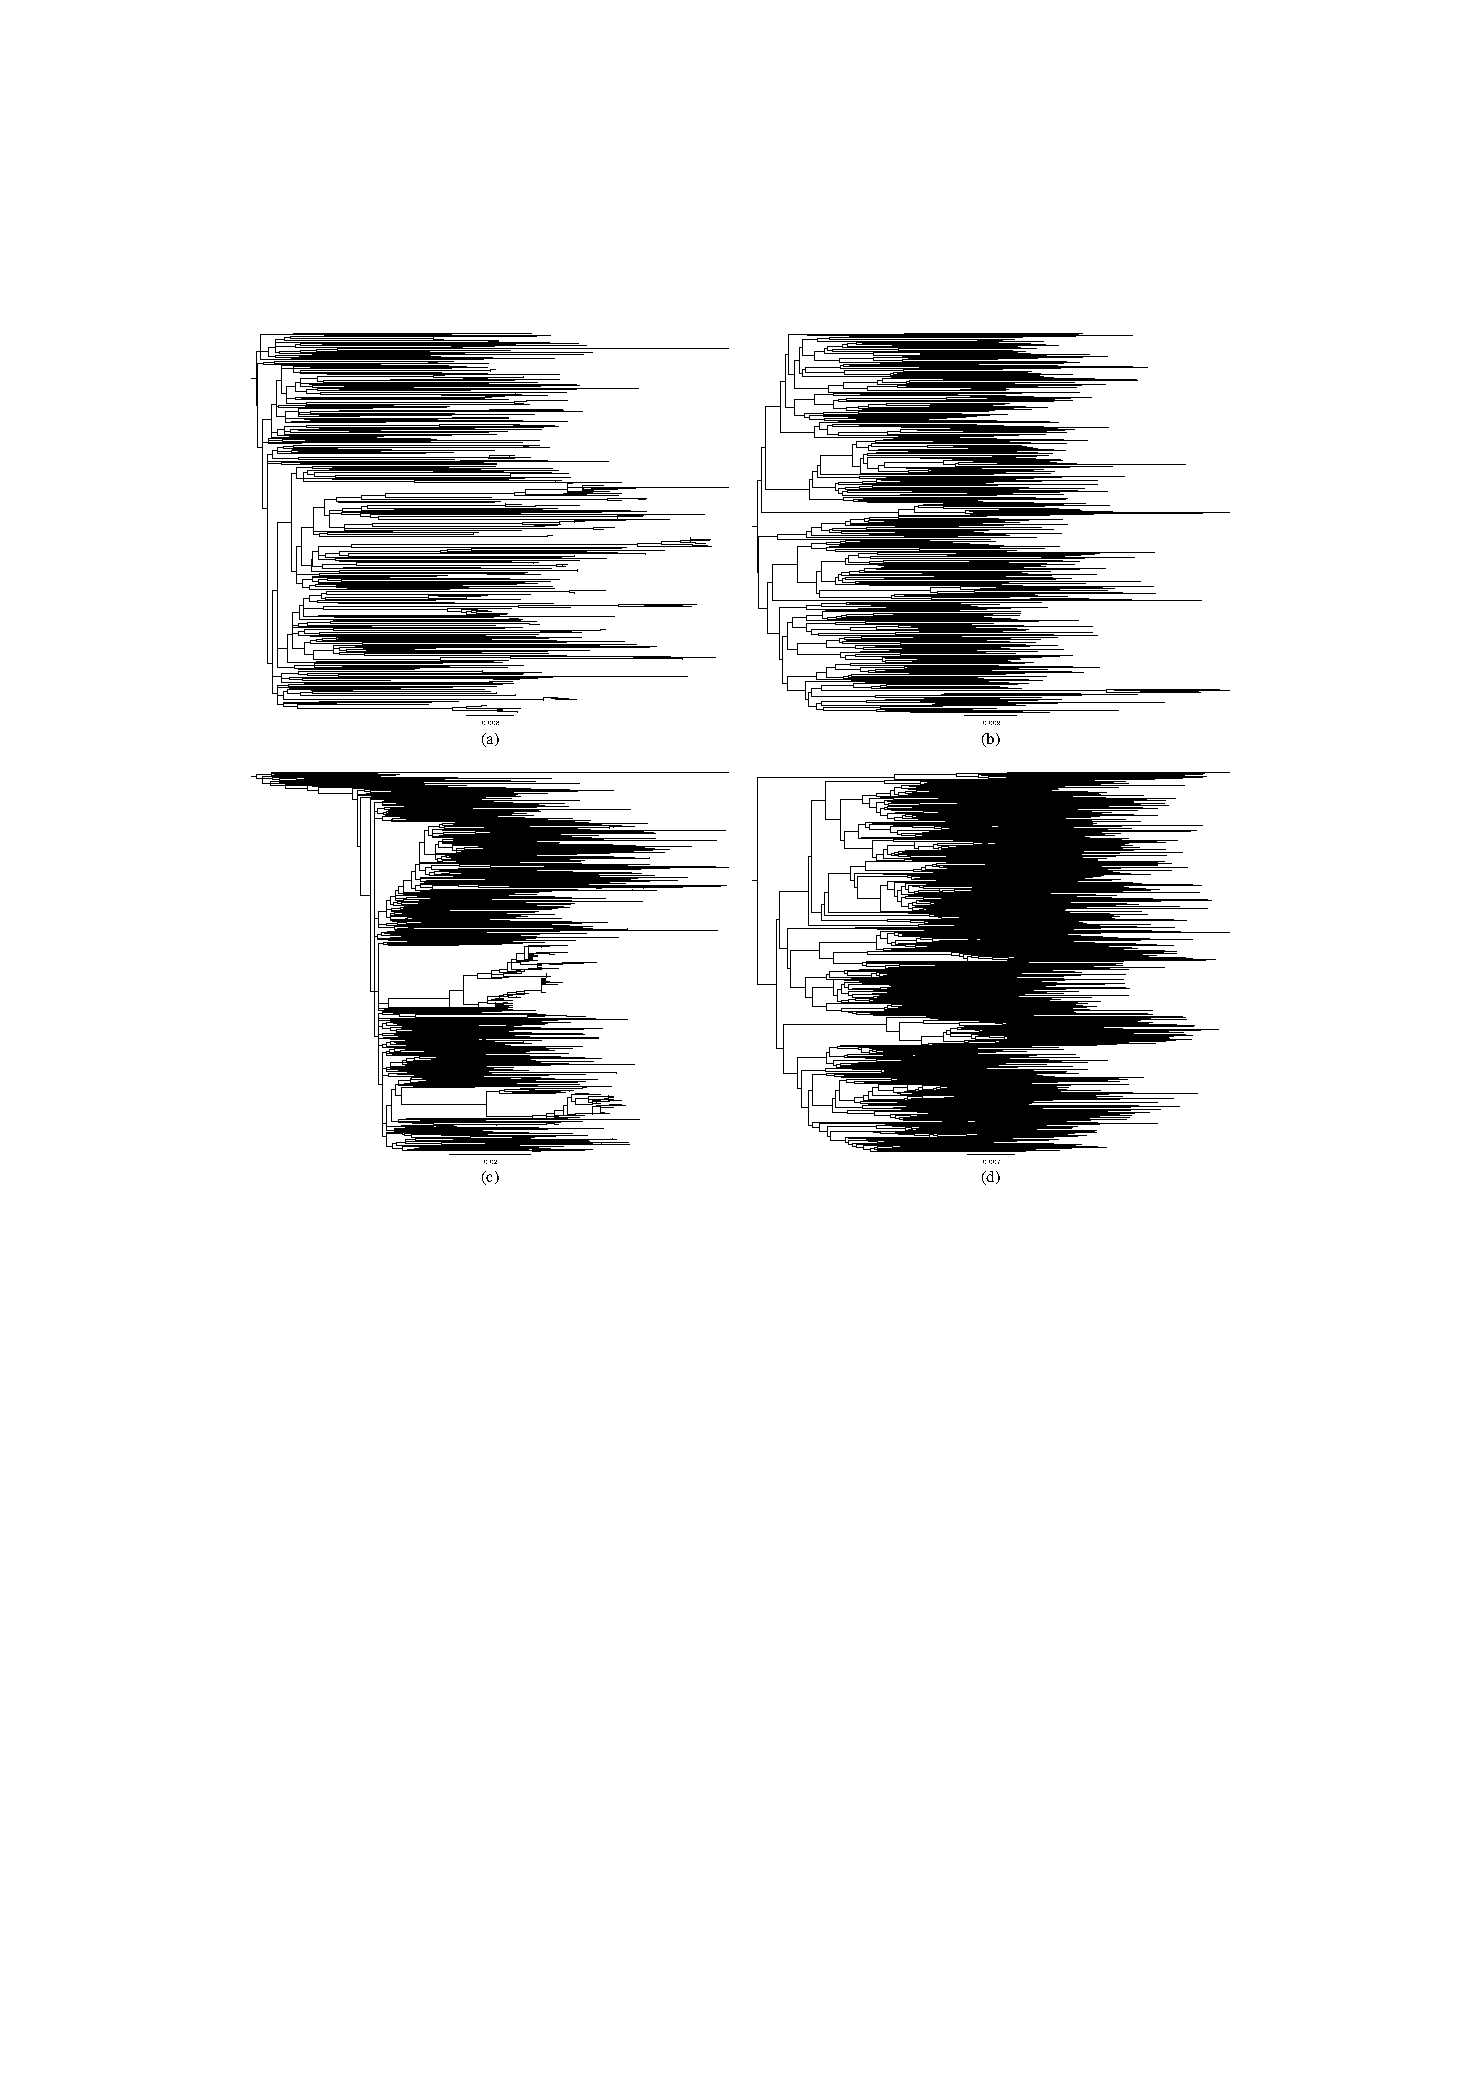
\includegraphics[width=\textwidth]{figs/favites-trees}
\caption[Real vs. Simulated Viral Phylogenies]
{Real versus simulated phylogenetic trees. Phylogenetic trees inferred from a real dataset of \textit{pol} sequences (a) from San Diego~\cite{Little2014}, (b) from a simulated San Diego dataset, (c) from the set of all \textit{pol} sequences in the \gls{LANL} \gls{HIV} database that were sampled in Uganda between 2005 and 2014, and (d) from a simulated Uganda dataset. Trees were inferred using the ModelFinder Plus feature~\cite{Kalyaanamoorthy2017} of IQ-TREE~\cite{Chernomor2016}.}
\label{fig:favites-trees}
\end{figure}

\begin{figure} % FIGURE S5 IN ORIGINAL PAPER
\centering
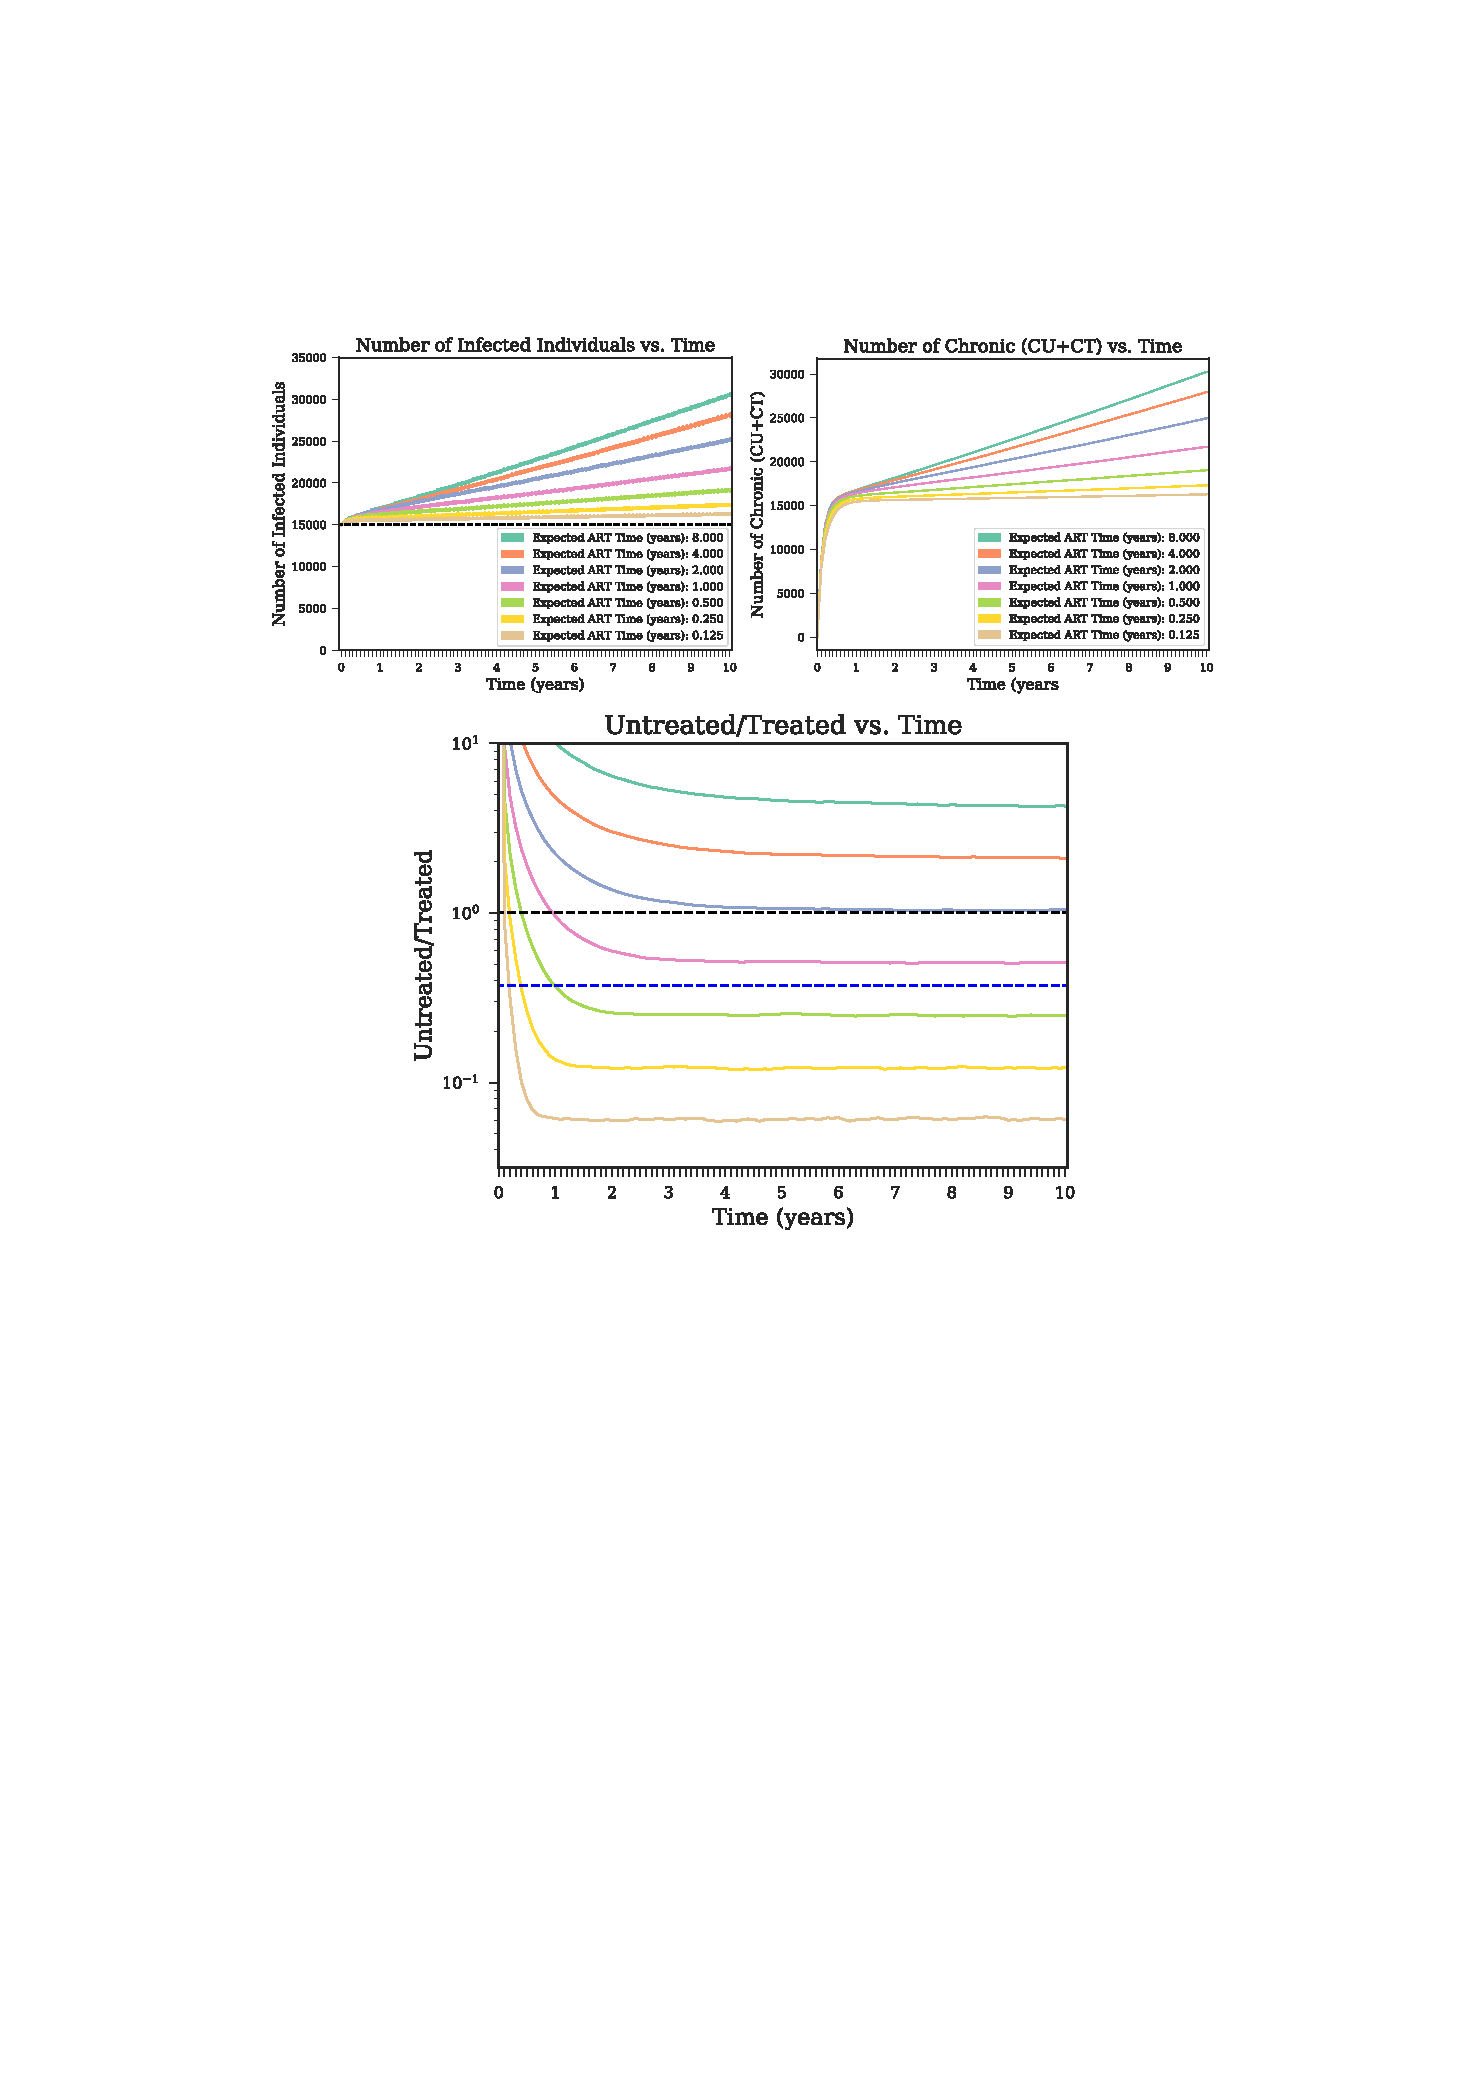
\includegraphics[width=\textwidth]{figs/favites-states-vs-time}
\caption[Epidemiological Model States vs. Time]
{Number of infected individuals vs. time for multiple rates of starting ART (colors). The underlying contact network was simulated using the base parameters listed in Table~\ref{tab:favites-params-main} with 100,000 total individuals and 15,000 seed individuals under the epidemiological model shown in Figure~\ref{fig:favites-model}. We show figures for all infected people (Top Left), and those in chronic states (Top Right). We also show (Bottom) the ratio of the number of untreated individuals vs. the number of treated individuals (log-scale) vs. time where untreated/treated = 1 is shown as a dashed black line, and the value of untreated/treated corresponding to the ``90-90-90'' goal~\cite{UNAIDS2017} is shown in blue.}
\label{fig:favites-states-vs-time}
\end{figure}

\begin{figure} % FIGURE S6 IN ORIGINAL PAPER
\centering
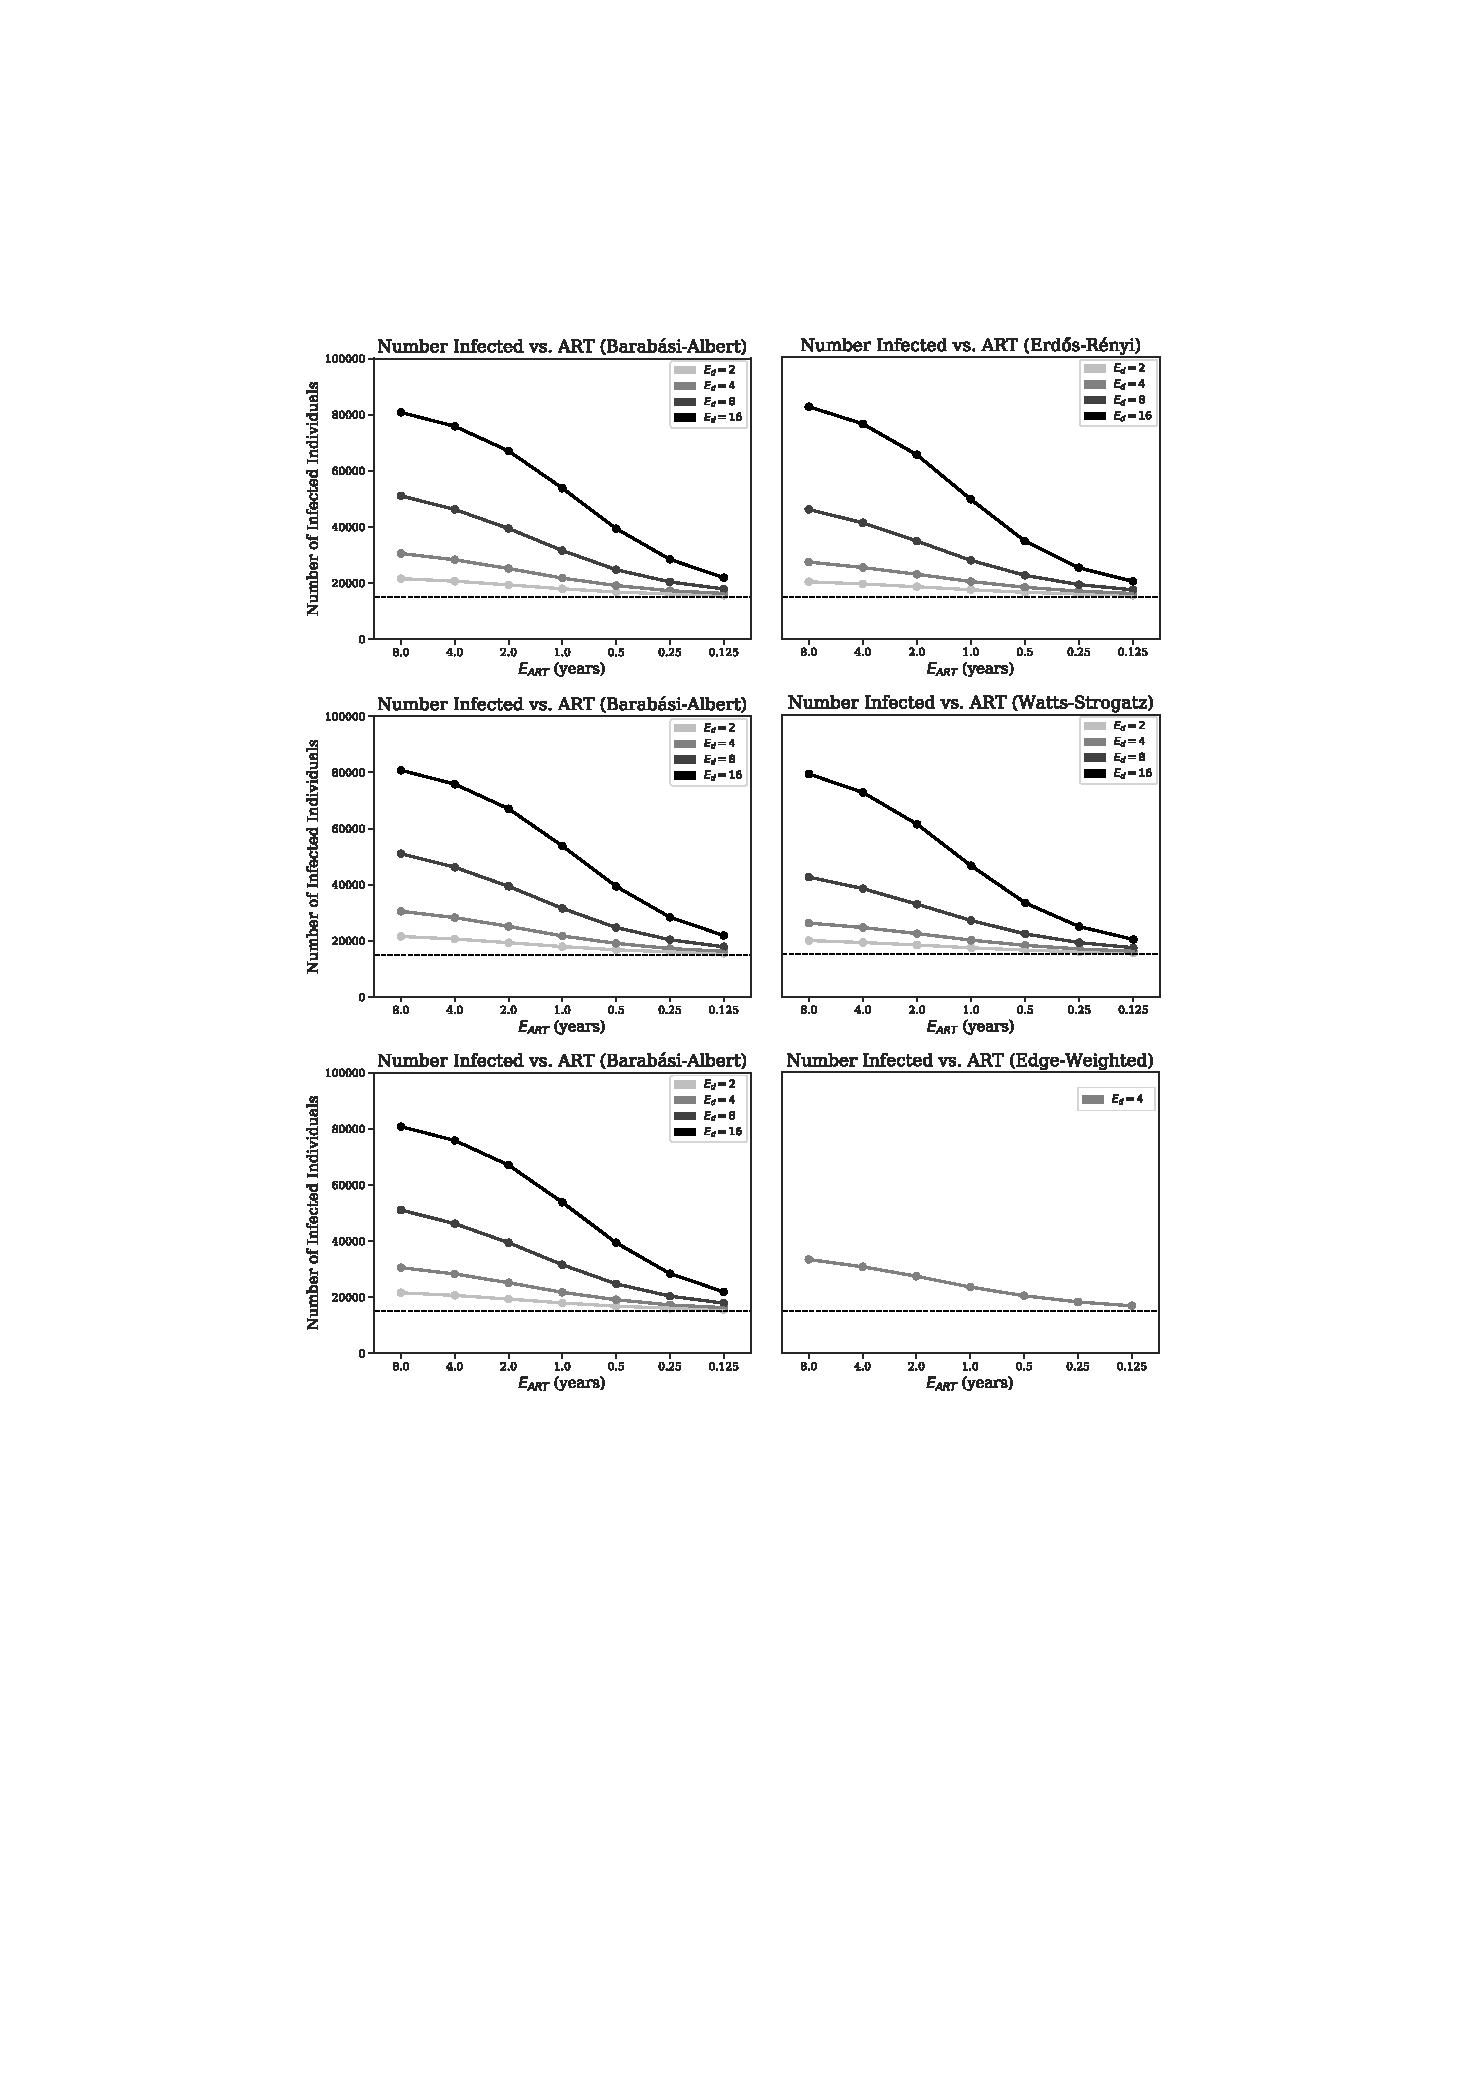
\includegraphics[width=0.9\textwidth]{figs/favites-num-infected-all}
\caption[Number of Infected Individuals vs. Expected Treatment Initiation Time]
{Total number of infected individuals vs. \EART for the \gls{BA}, \gls{ER}, and \gls{WS} models with random seed selection as well as for the \gls{BA} model with edge-weighted seed selection with various expected degrees. The base parameters were chosen for all other parameters. The number of seed individuals (15,000) is shown by a black dashed line. The BA figure is repeated in each row on the left to facilitate visual comparison to other models.}
\label{fig:favites-num-infected-all}
\end{figure}

\begin{figure} % FIGURE S7 IN ORIGINAL PAPER
\centering
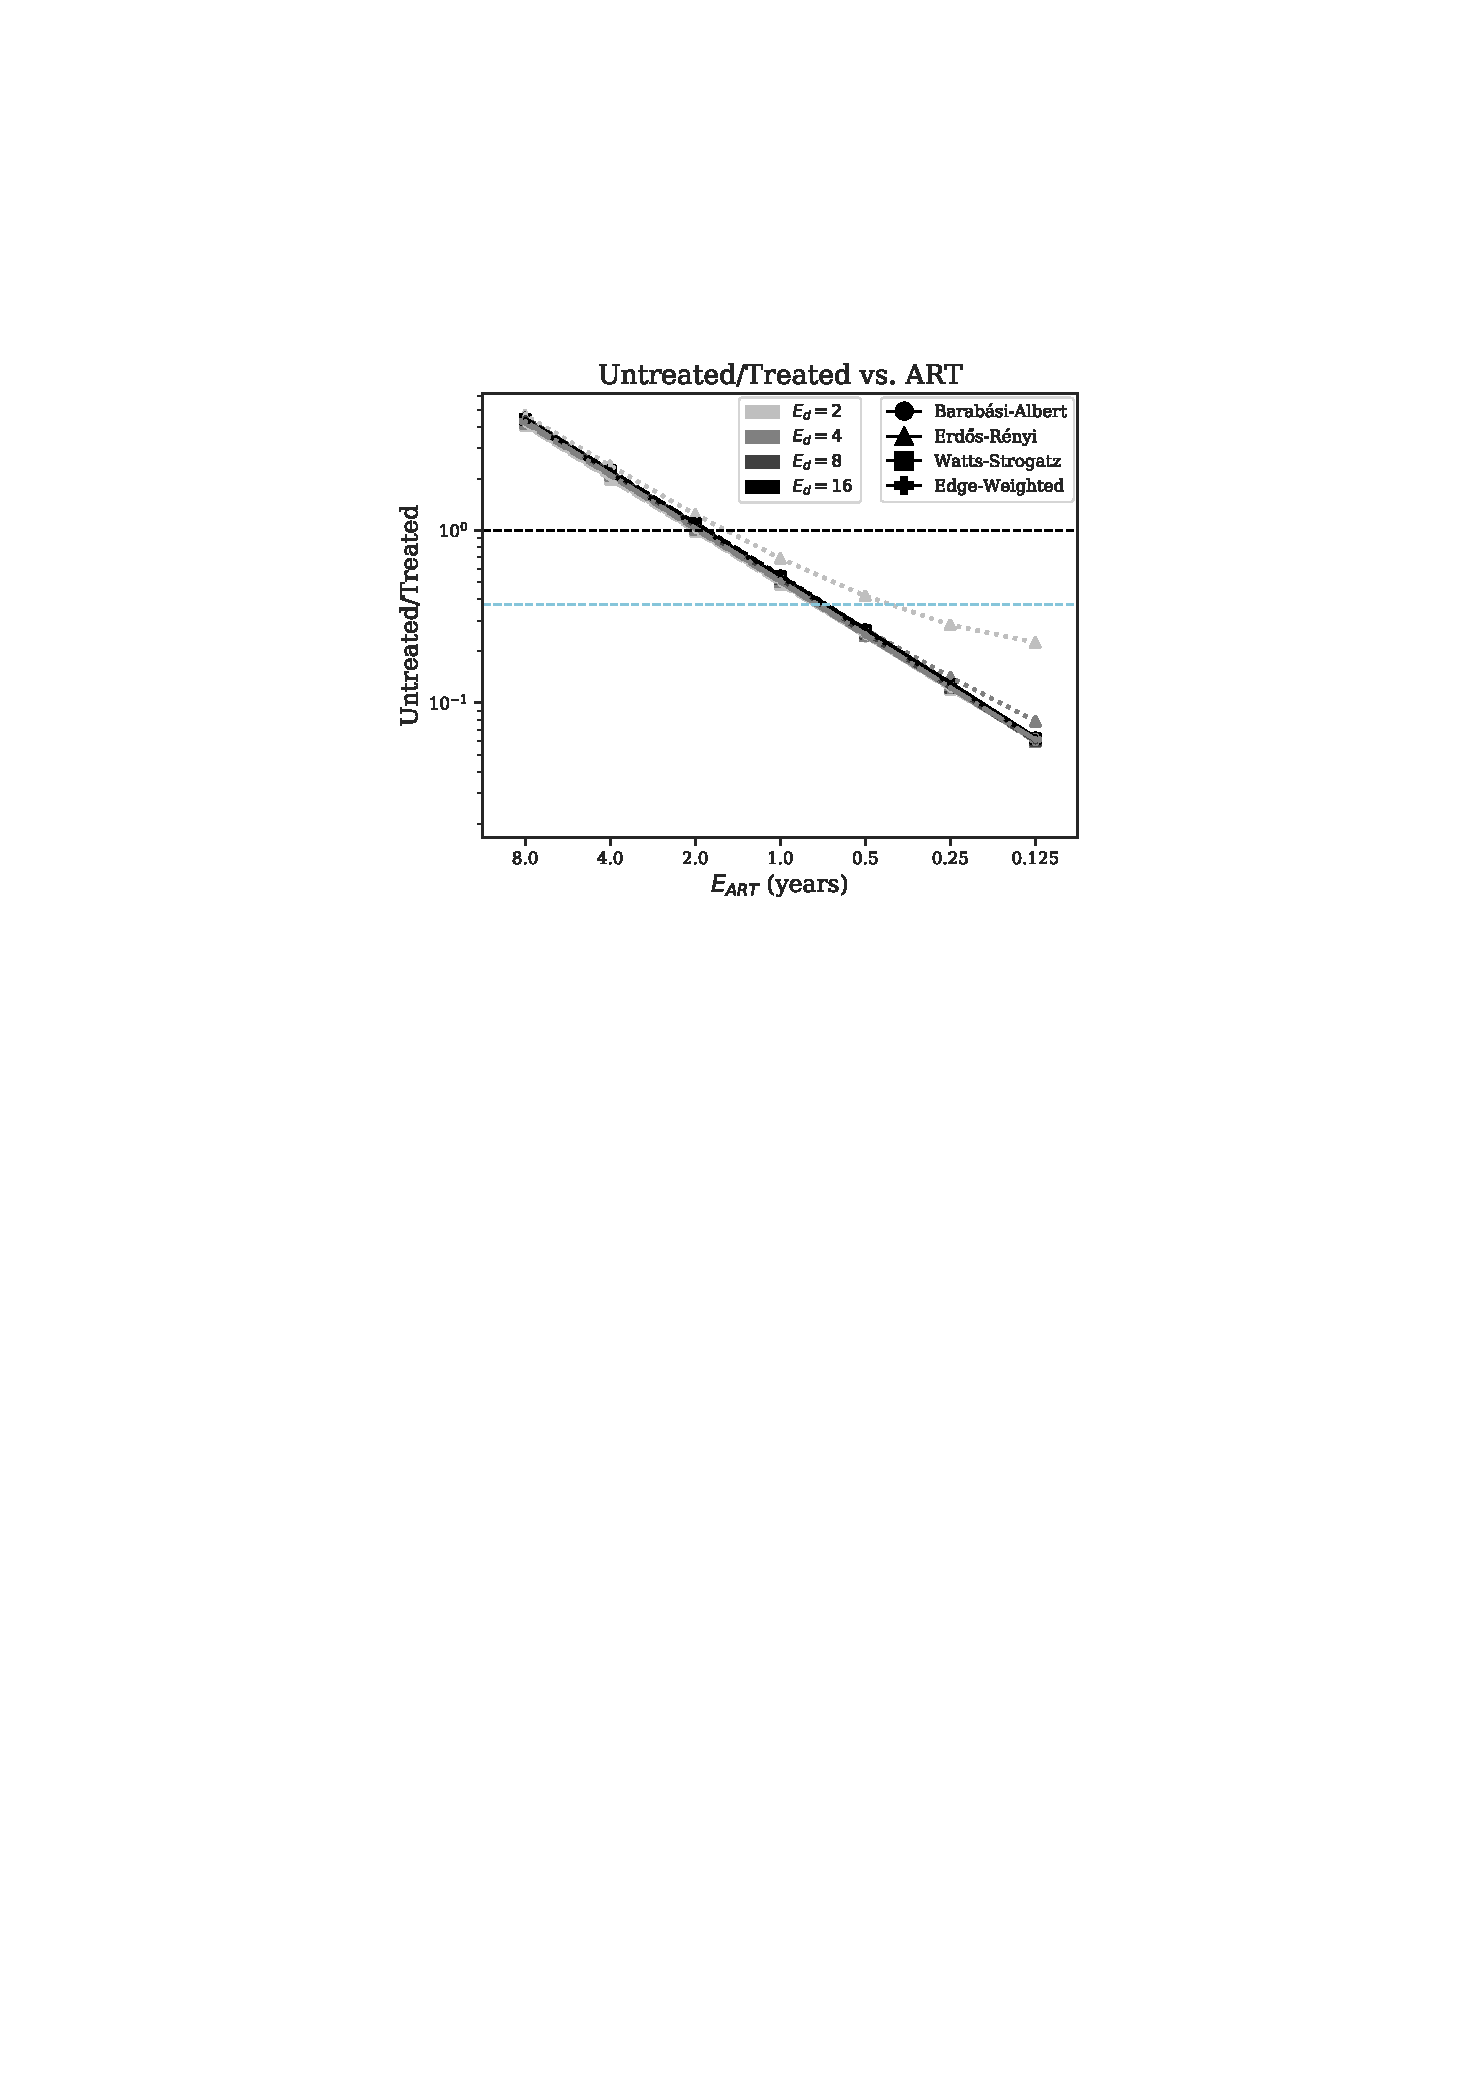
\includegraphics[width=0.55\textwidth]{figs/favites-untreated-vs-treated-all}
\caption[Treated to Untreated Ratio vs. Expected Treatment Initiation Time]
{The ratio of the number of untreated vs. the number of treated individuals (log-scale) vs. expected time to begin Antiretroviral Therapy (\EART) for the \gls{BA} (solid circles), \gls{ER} (dotted triangles), and \gls{WS} models (dashed squares) with random seed selection as well as the \gls{BA} with edge-weighted seed selection (dot-dashed pluses) with various \ED values (colors). Untreated/treated = 1 is shown as a dashed black line, and the value of untreated/treated corresponding to the ``90-90-90'' goal~\cite{UNAIDS2017} is shown as a dashed blue line $\left(\frac{1-0.9^3}{0.9^3}\approx0.37\right)$.}
\label{fig:favites-untreated-vs-treated-all}
\end{figure}

\begin{figure} % FIGURE S8 IN ORIGINAL PAPER
\centering
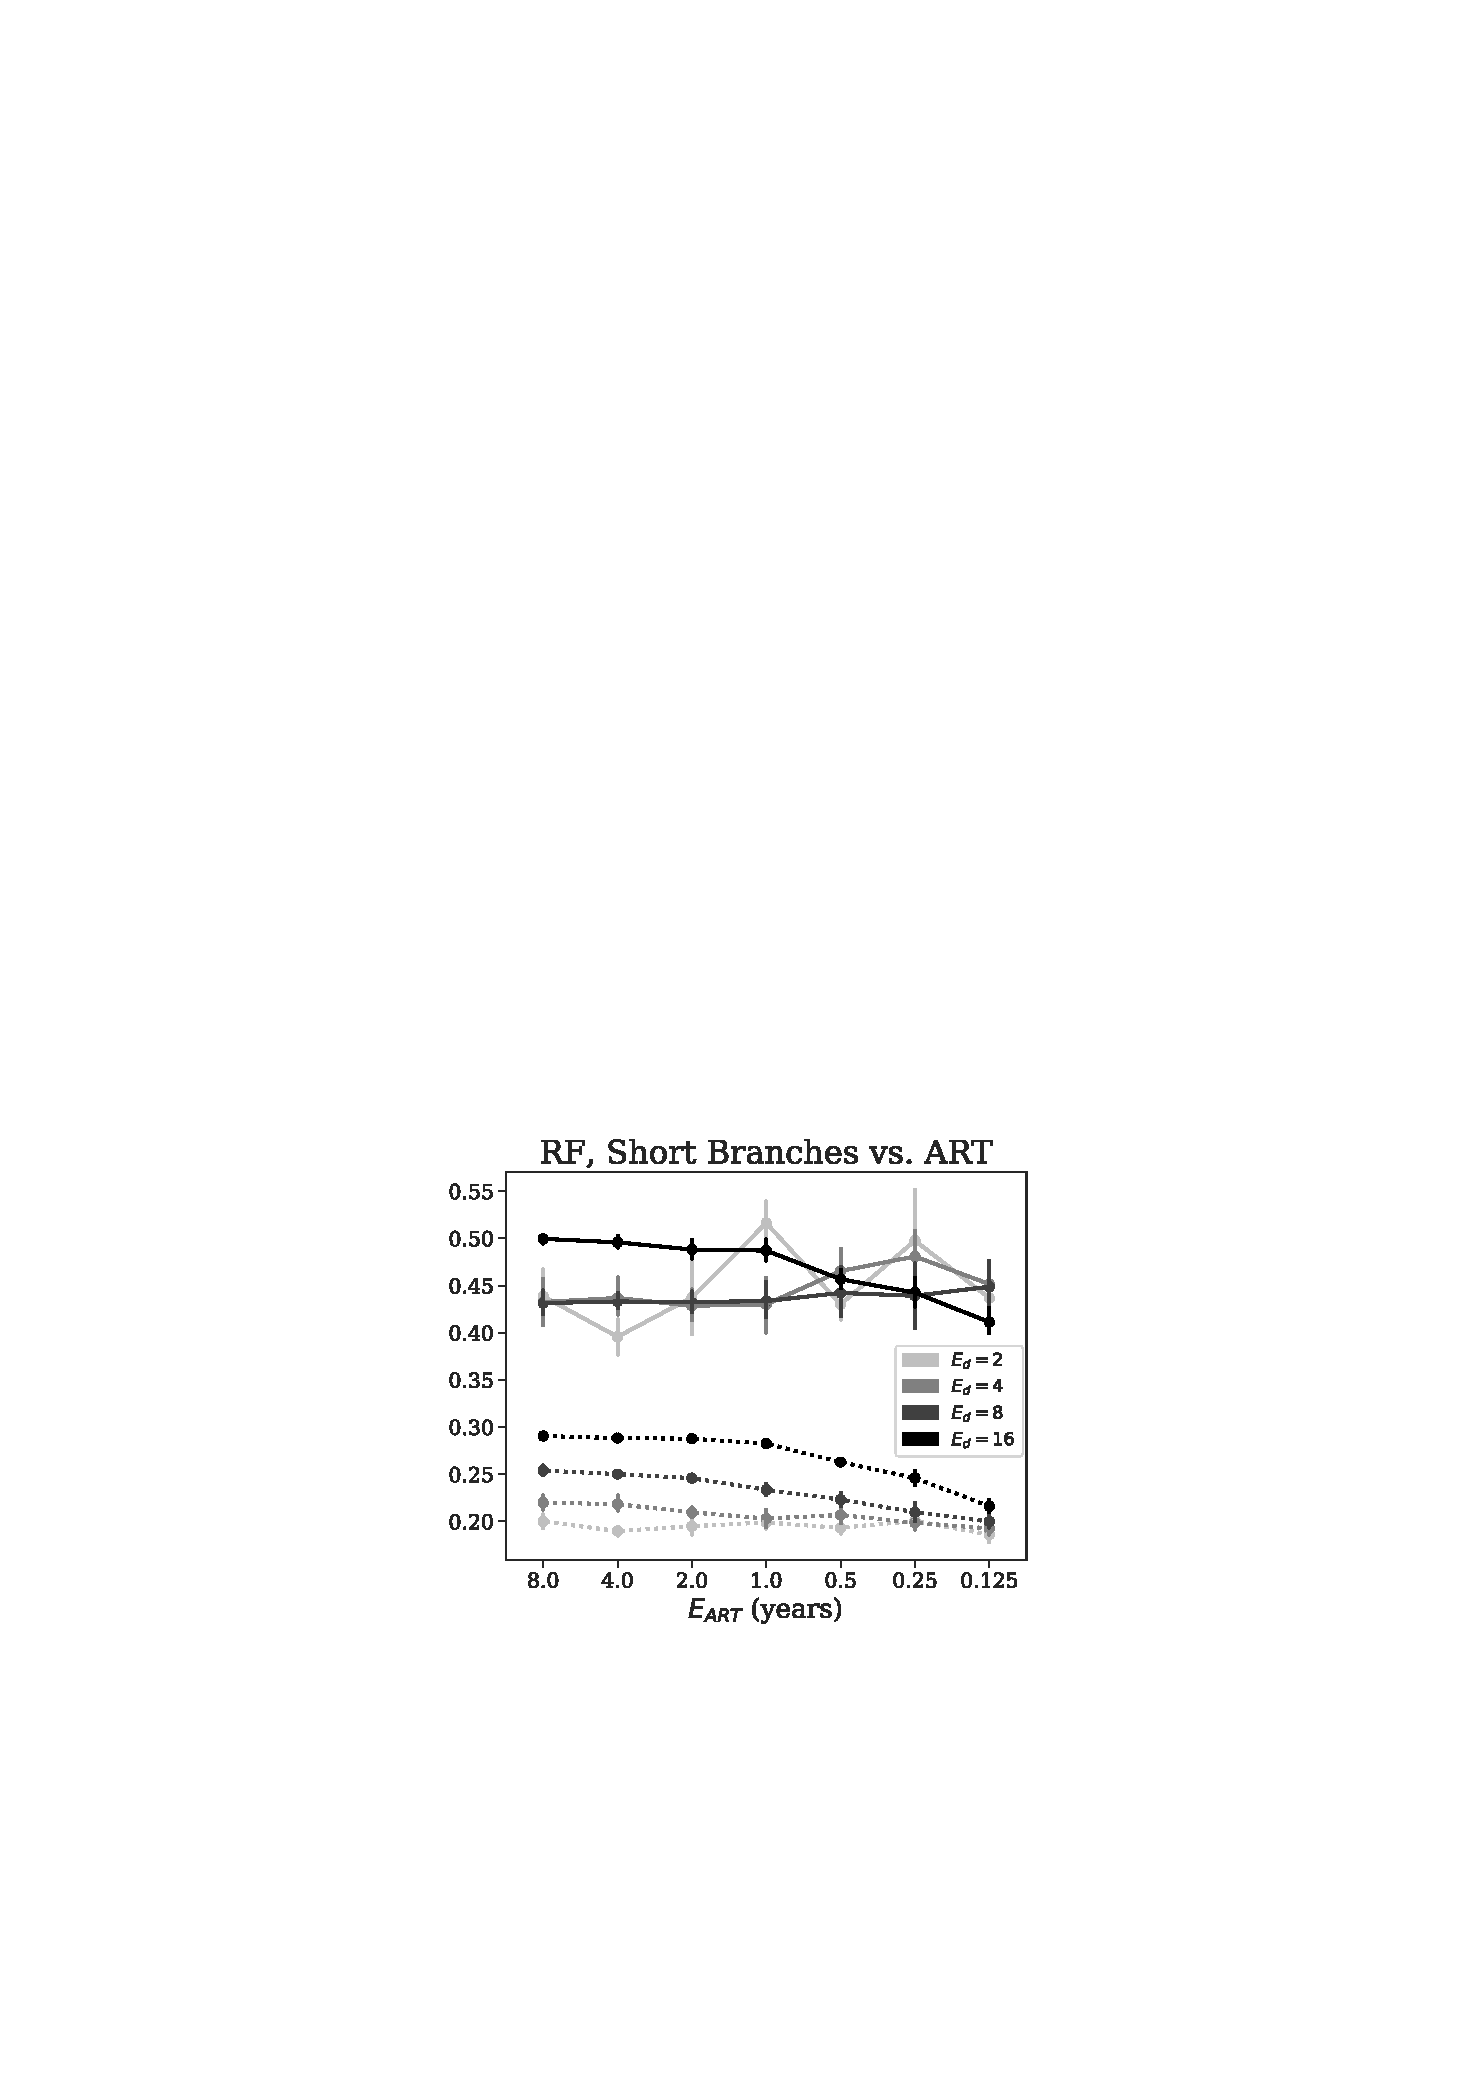
\includegraphics[width=0.55\textwidth]{figs/favites-rf-short-vs-art}
\caption[Topology Error and Short Branches vs. Expected Treatment Initiation Time]
{\gls{RF} distance (solid lines) and proportion of ``extremely short'' branches (dotted lines) vs. expected time to begin Antiretroviral Therapy (\EART) for the \gls{BA} model with various \ED values (colors) with all other parameters set to base values. We define branches to be ``extremely short'' if the expected number of mutations along the branch is less than or equal to 1 (i.e., the branch length is less than or equal to the reciprocal of the sequence length). All the trees are inferred using FastTree~2 and \gls{RF} is computed with respect to the true tree.}
\label{fig:favites-rf-short-vs-art}
\end{figure}

%% END FAVITES SUPPLEMENT